\documentclass[12pt]{article}

\usepackage[utf8]{inputenc}
\usepackage{graphicx}
\usepackage{float}
\usepackage{amsmath}
\usepackage{placeins}
\usepackage{gensymb}
\usepackage{caption}
\usepackage{subcaption}


\usepackage[letterpaper,margin=0.75in]{geometry}
\graphicspath{images/}
\begin{document}
\begin{titlepage}
\begin{center}
% Upper part of the page
\vbox{}
\vbox{}
\vbox{}
\vbox{}
\vbox{}
\vbox{}
\vbox{}
\vbox{}
\vbox{}

\includegraphics[width=0.75\textwidth]{Images/ubc.png}\\[0.5cm]
\textrm{Martin Alejo}\\[0.5cm]
\catcode`#=12
\textrm{#75296665}\\[0.5cm]
\textrm{December 9, 2022}\\[0.5cm]
\textrm{Mini Project 4}\\[0.5cm]
\textrm{University of British Columbia}\\[0.5cm]
\textrm{Electrical and Computer Engineering}\\[0.5cm]
\textrm{ELEC 301}\\[0.5cm]
\textrm{Instructor: Nicolas Jaeger}\\[0.5cm]

\includegraphics[width=0.18\textwidth]{Images/Signature.png}\\[0.5cm]
\vbox{ }
\end{center}
\end{titlepage}
\pagebreak
\pagenumbering{roman}
\tableofcontents
\pagebreak
\listoffigures
\listoftables
\pagebreak
\pagenumbering{arabic}


\section{Introduction}
For this project, we will be using SPICE software to simulate active filters and oscillators.
\section{Part A}
\subsubsection{Part 1}
For this part, we will be designing a 2nd order Butterworth low pass active filter using the UA741 operational amplifier. 
Here is the circuit that we will be using for this part:

\begin{figure}[H]
    \centering
    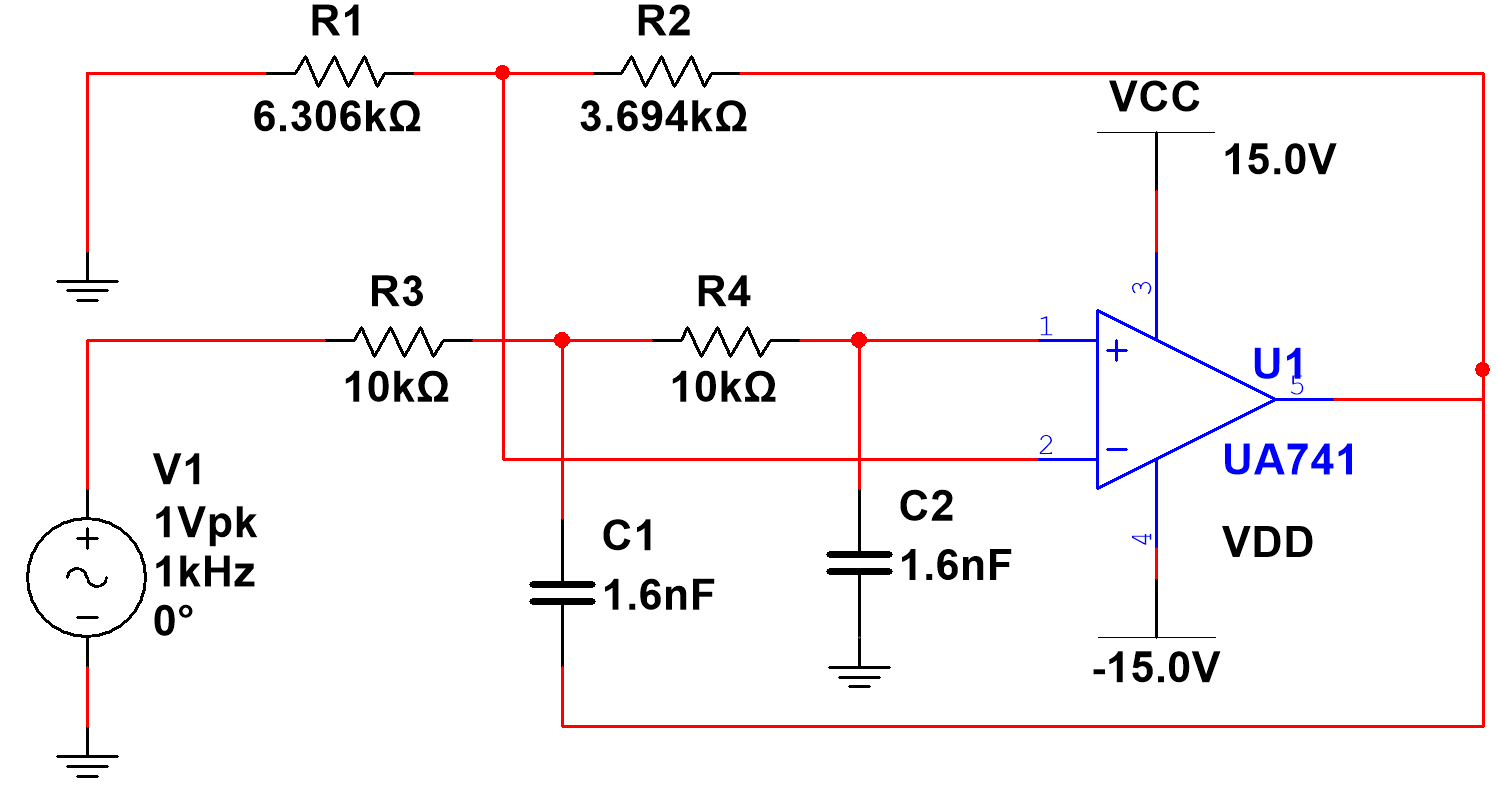
\includegraphics[height=0.2\textwidth]{Images/partAcircuit.png}\\
    \caption{Second Order Butterworth Filter}
    \label{fig:SecondOrderButterworthFilter}
\end{figure}

The calculations to find the resistance $R_1$,$R_2$ and capacitance C, we will be using the formulas from the class notes [1].  
The formulas can also be found from no. 1 in the Appendix. From the formulas, we can see that

\begin{center}
\boxed{R_1 = 6.306k \Omega, R_2 = 3.694k\Omega, C = 1.6nF, A_m = 1.59\frac{V}{V}}
\end{center}
Below is the phase and magnitude plot for our filter:

\begin{figure}[H]
    \centering
    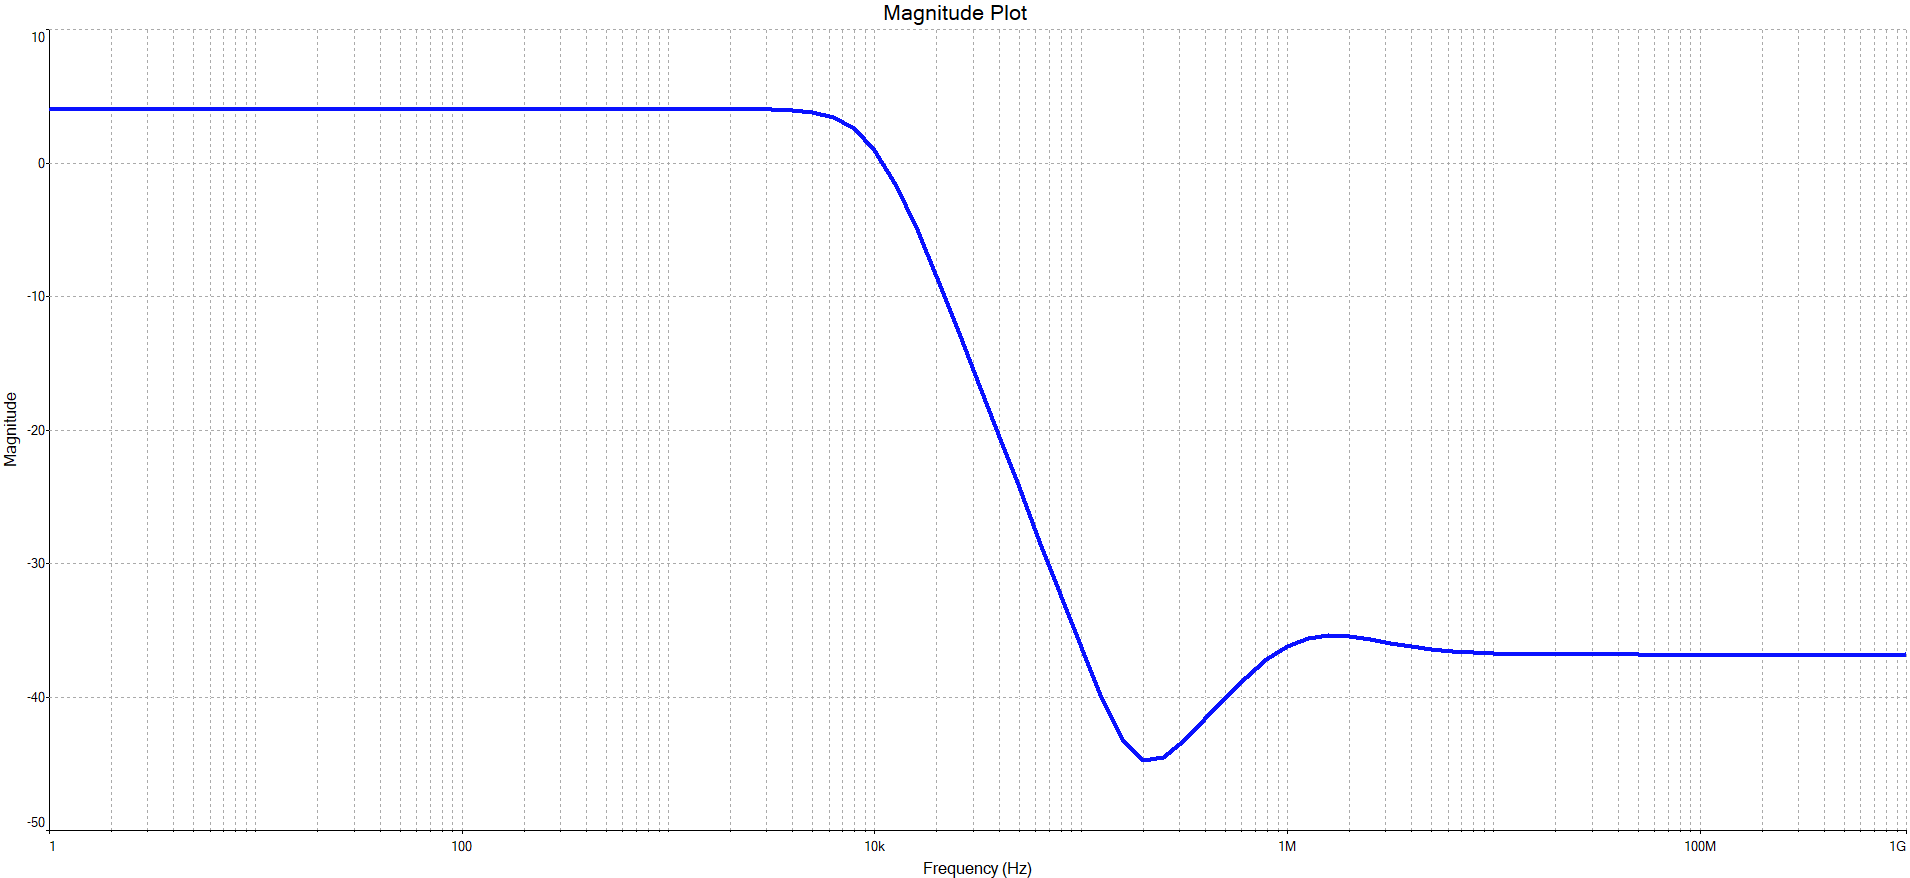
\includegraphics[height=0.4\textwidth]{Images/magnitude_plot.png}\\
    \caption{Bode Magnitude Plot}
    \label{fig:magntitudeplot}
\end{figure}


\begin{figure}[H]
    \centering
    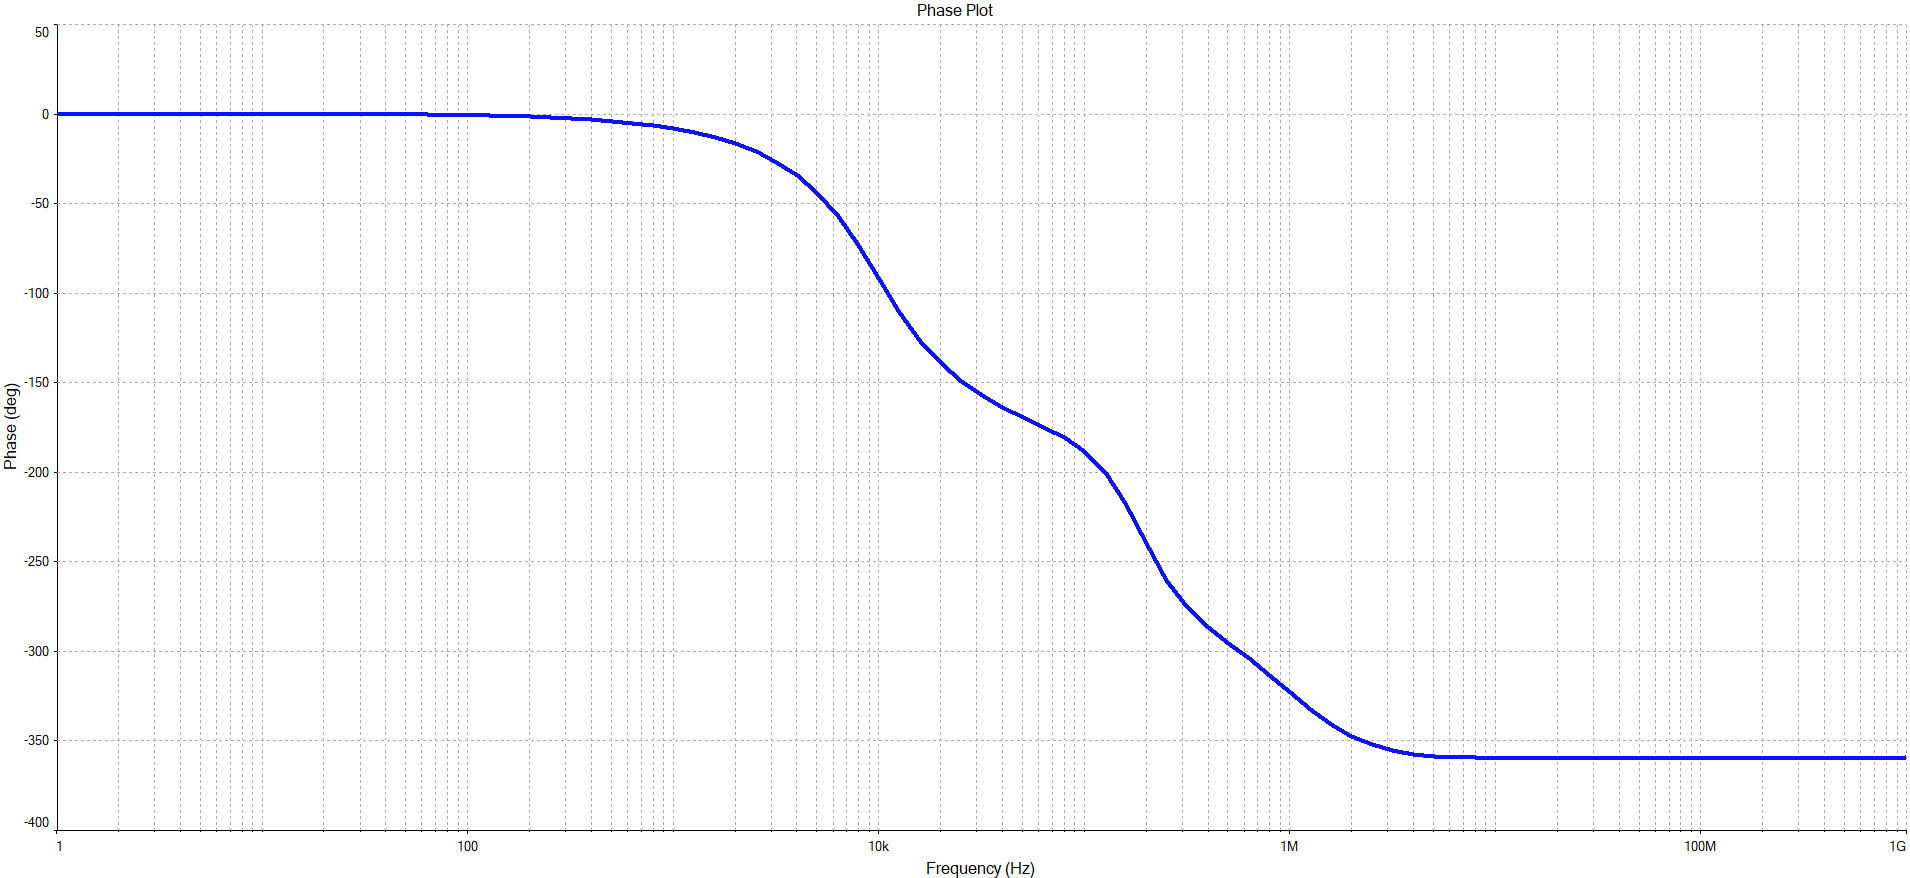
\includegraphics[height=0.4\textwidth]{Images/phase_plot.png}\\
    \caption{Bode Phase Plot}
    \label{fig:phaseplot}
\end{figure}


\subsubsection{Part 2}
For this part, we will be grounding the input, and measuring the output of the OpAmp.
To determine the value of $A_m$ when the circuit begins to oscillate, we need the transfer fucntion. The function is shown below,
where R = $10k\Omega$ and C is the value found previously:
\begin{flalign}
&H(s) = A_M\frac{\frac{1}{(RC)^2}}{s^2+s\frac{3-A_M}{RC}+\frac{1}{(RC)^2}}\nonumber
\end{flalign}
Changing the values of the resistances, we find that the oscillations occour when $R_1=3k\Omega$ and $R_2 =
7k\Omega$.
The oscillation is shown below:
\begin{figure}[H]
    \centering
    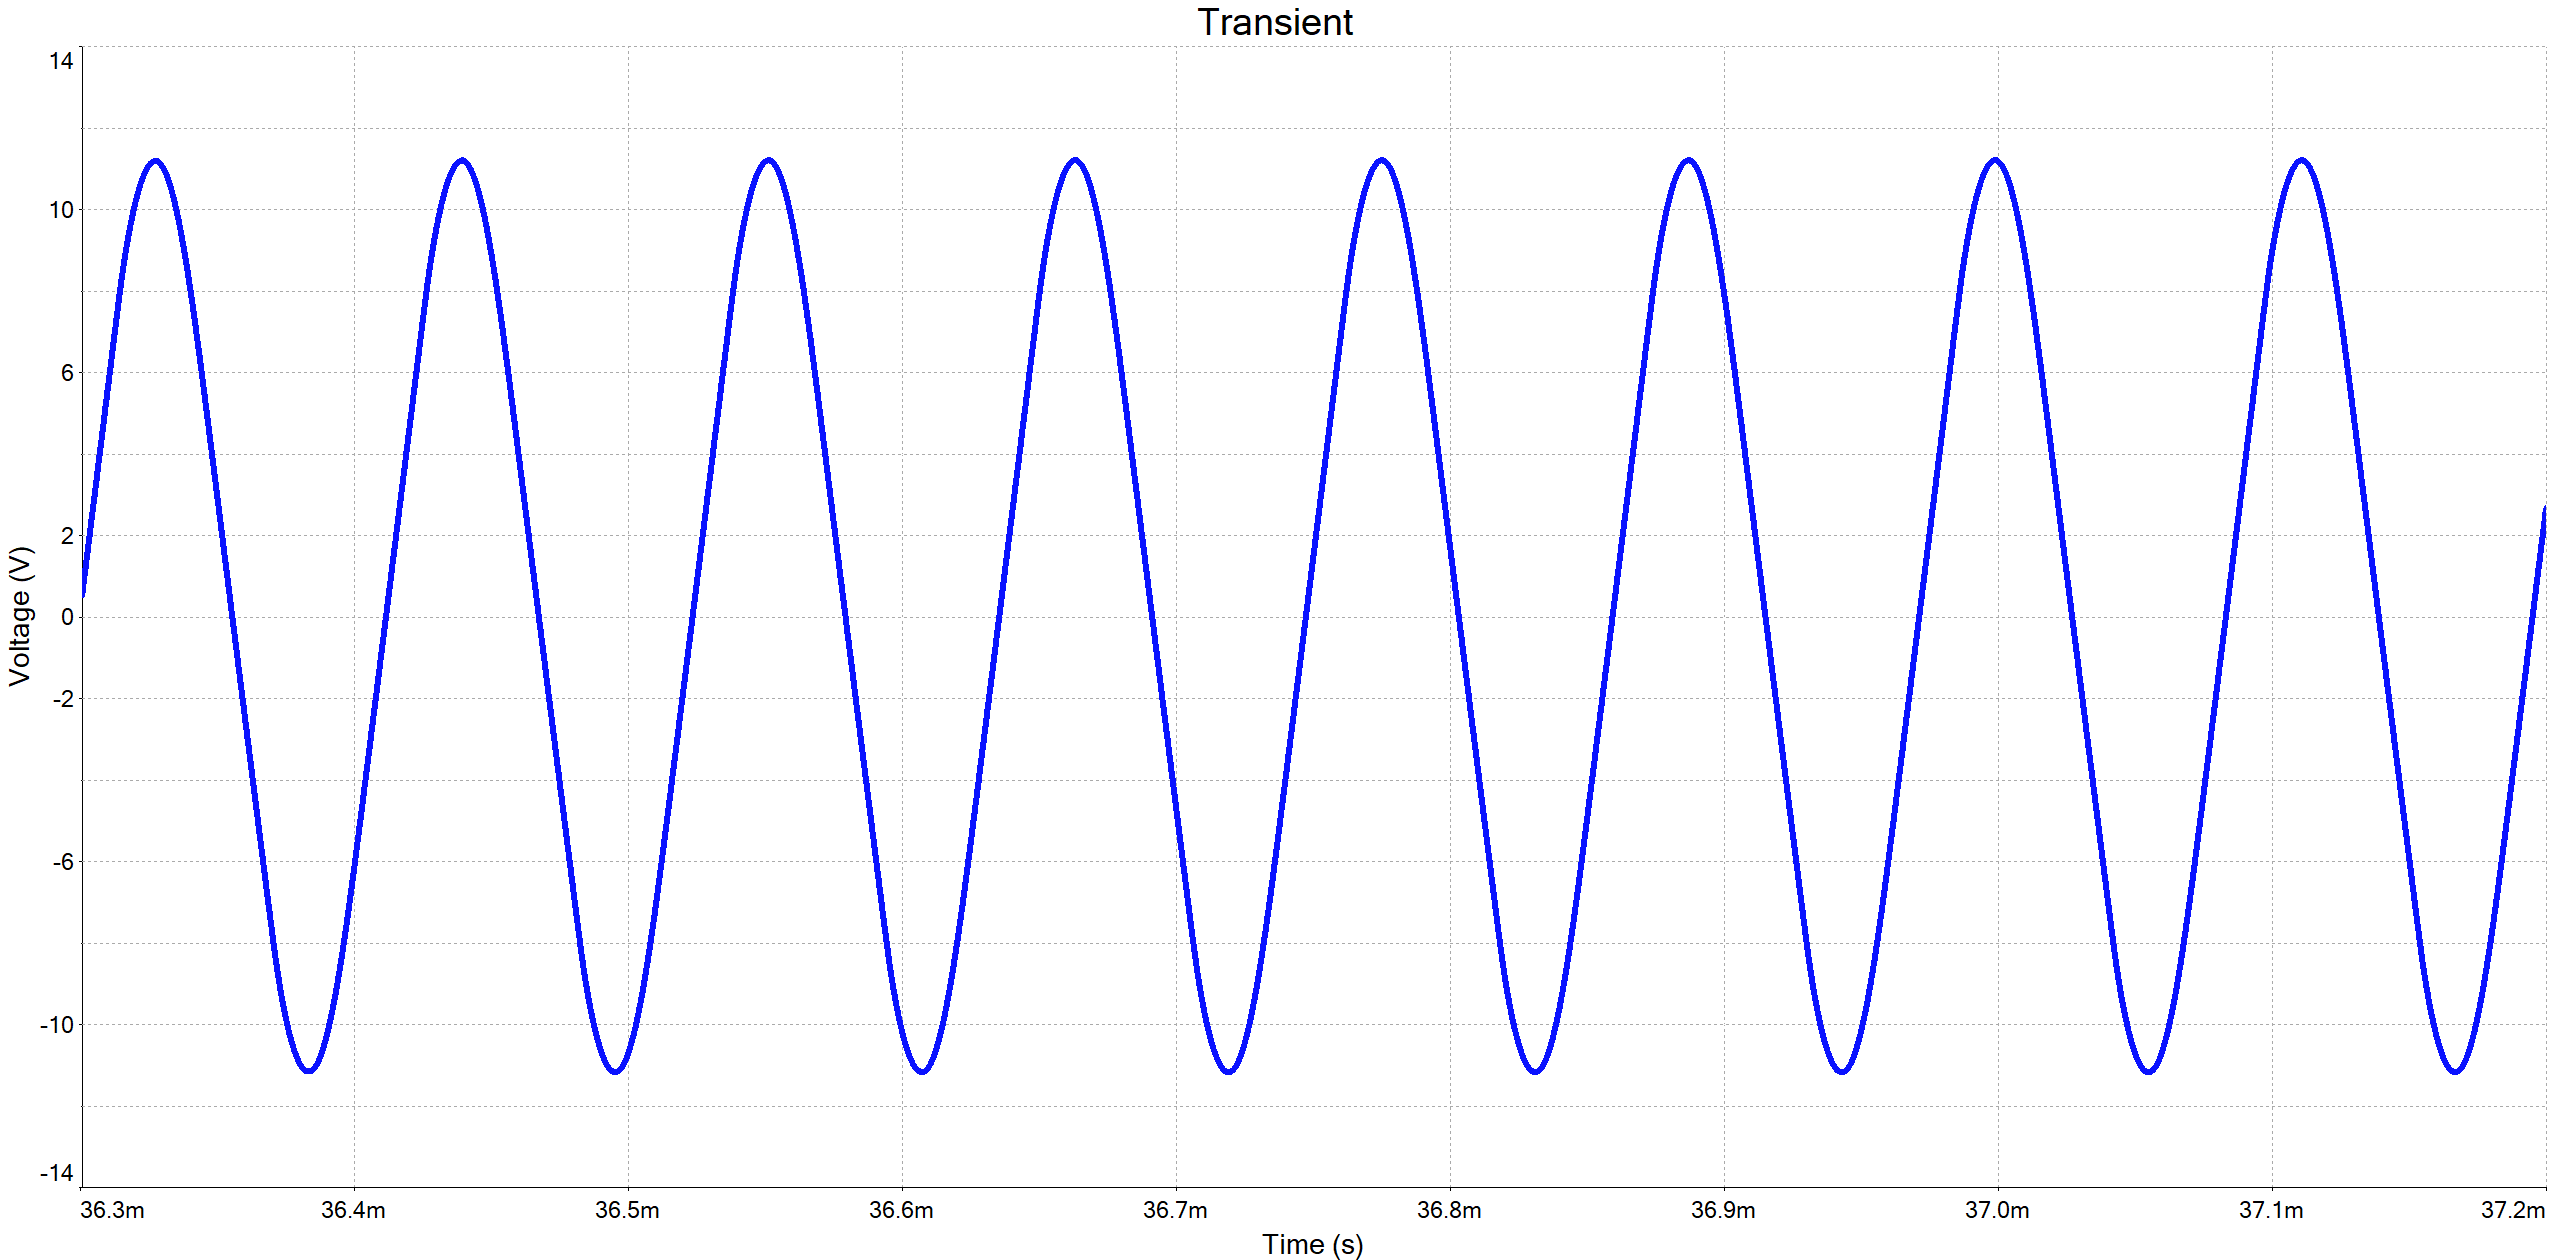
\includegraphics[height=0.32\textwidth]{Images/partatransient.png}\\
    \caption{Oscillating Output}
    \label{fig:oscillatingoutput}
\end{figure}
\FloatBarrier
Below is the root locus plot:

\begin{figure}
\centering
\begin{minipage}{.5\textwidth}
    \centering
    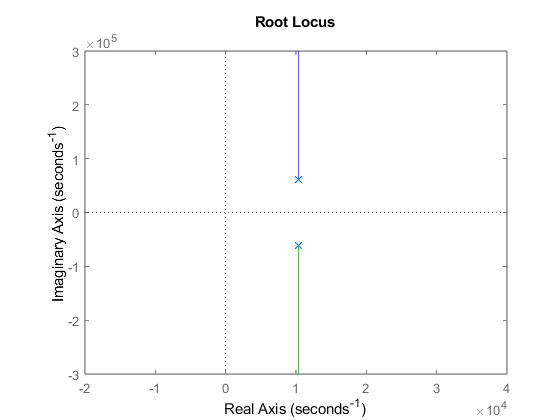
\includegraphics[height=0.7\textwidth]{Images/unstablerootlocus.png}\\
    \caption{Unstable Root Locus Plot}
    \label{fig:unstablerootlocus}
\end{minipage}%
\begin{minipage}{.5\textwidth}
    \centering
    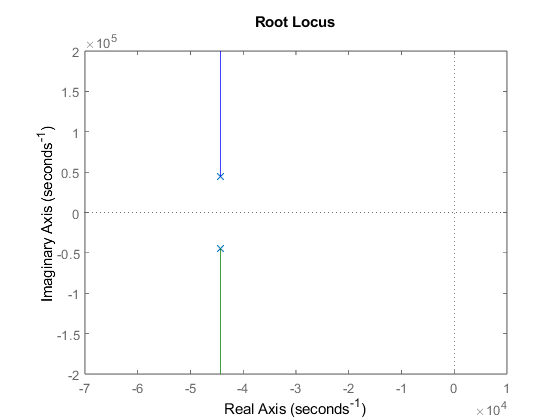
\includegraphics[height=0.7\textwidth]{Images/stablerootlocus.png}\\
    \caption{Stable Root Locus Plot}
    \label{fig:rootlocus}
\end{minipage}
\end{figure}
\FloatBarrier
The root locus plot where $A_M>3$ and $A_M<3$ is Figure \ref{fig:unstablerootlocus} and Figure \ref{fig:rootlocus} respectively. 
We can see from the plot that when the oscillations occour, $A_M$ is greater than 3. This would then cause the system to be 
unstable as shown in Figure \ref{fig:unstablerootlocus}, since the poles are on the right side on the $jw$ axis. When the
poles are on the other side of the $jw$ axis, the system is stable, and doesn't cause the output to oscillate. This happens
when $A_M<3$. The reason why it has to be less than 3 for the system to be stable is because of the characteristic equation in the transfer function. 
If $A_M$ is greater than 3, it causes one of the coefficients in the characteristic equation to be negative, causing instability
in the system.












\section{Part B}
\section{Part C}

\section{Appendix}
\begin{flalign}
    &k = 3 - \sqrt(2)\\
\end{flalign}
\section{References}
1. ELEC 301 Class notes 
\newline
2. Mini Project 4 Document
\newline
3. Standard Resistor and Capacitor Values (Canvas)
\newline
4. Circuit Maker SPICE Model


\end{document}